% вариант сделан специально для тренировочного экзамена 2026.04.04, автор: Горелова

\samerowans{\begin{problem}{1 (1 балл)}
$KE$ --- биссектриса $\angle{CKB}$, $\angle{CKE} = 40^{\text{o}}$, $DK \perp CK$. Найдите $\angle{AKD}$.
\end{problem}} 

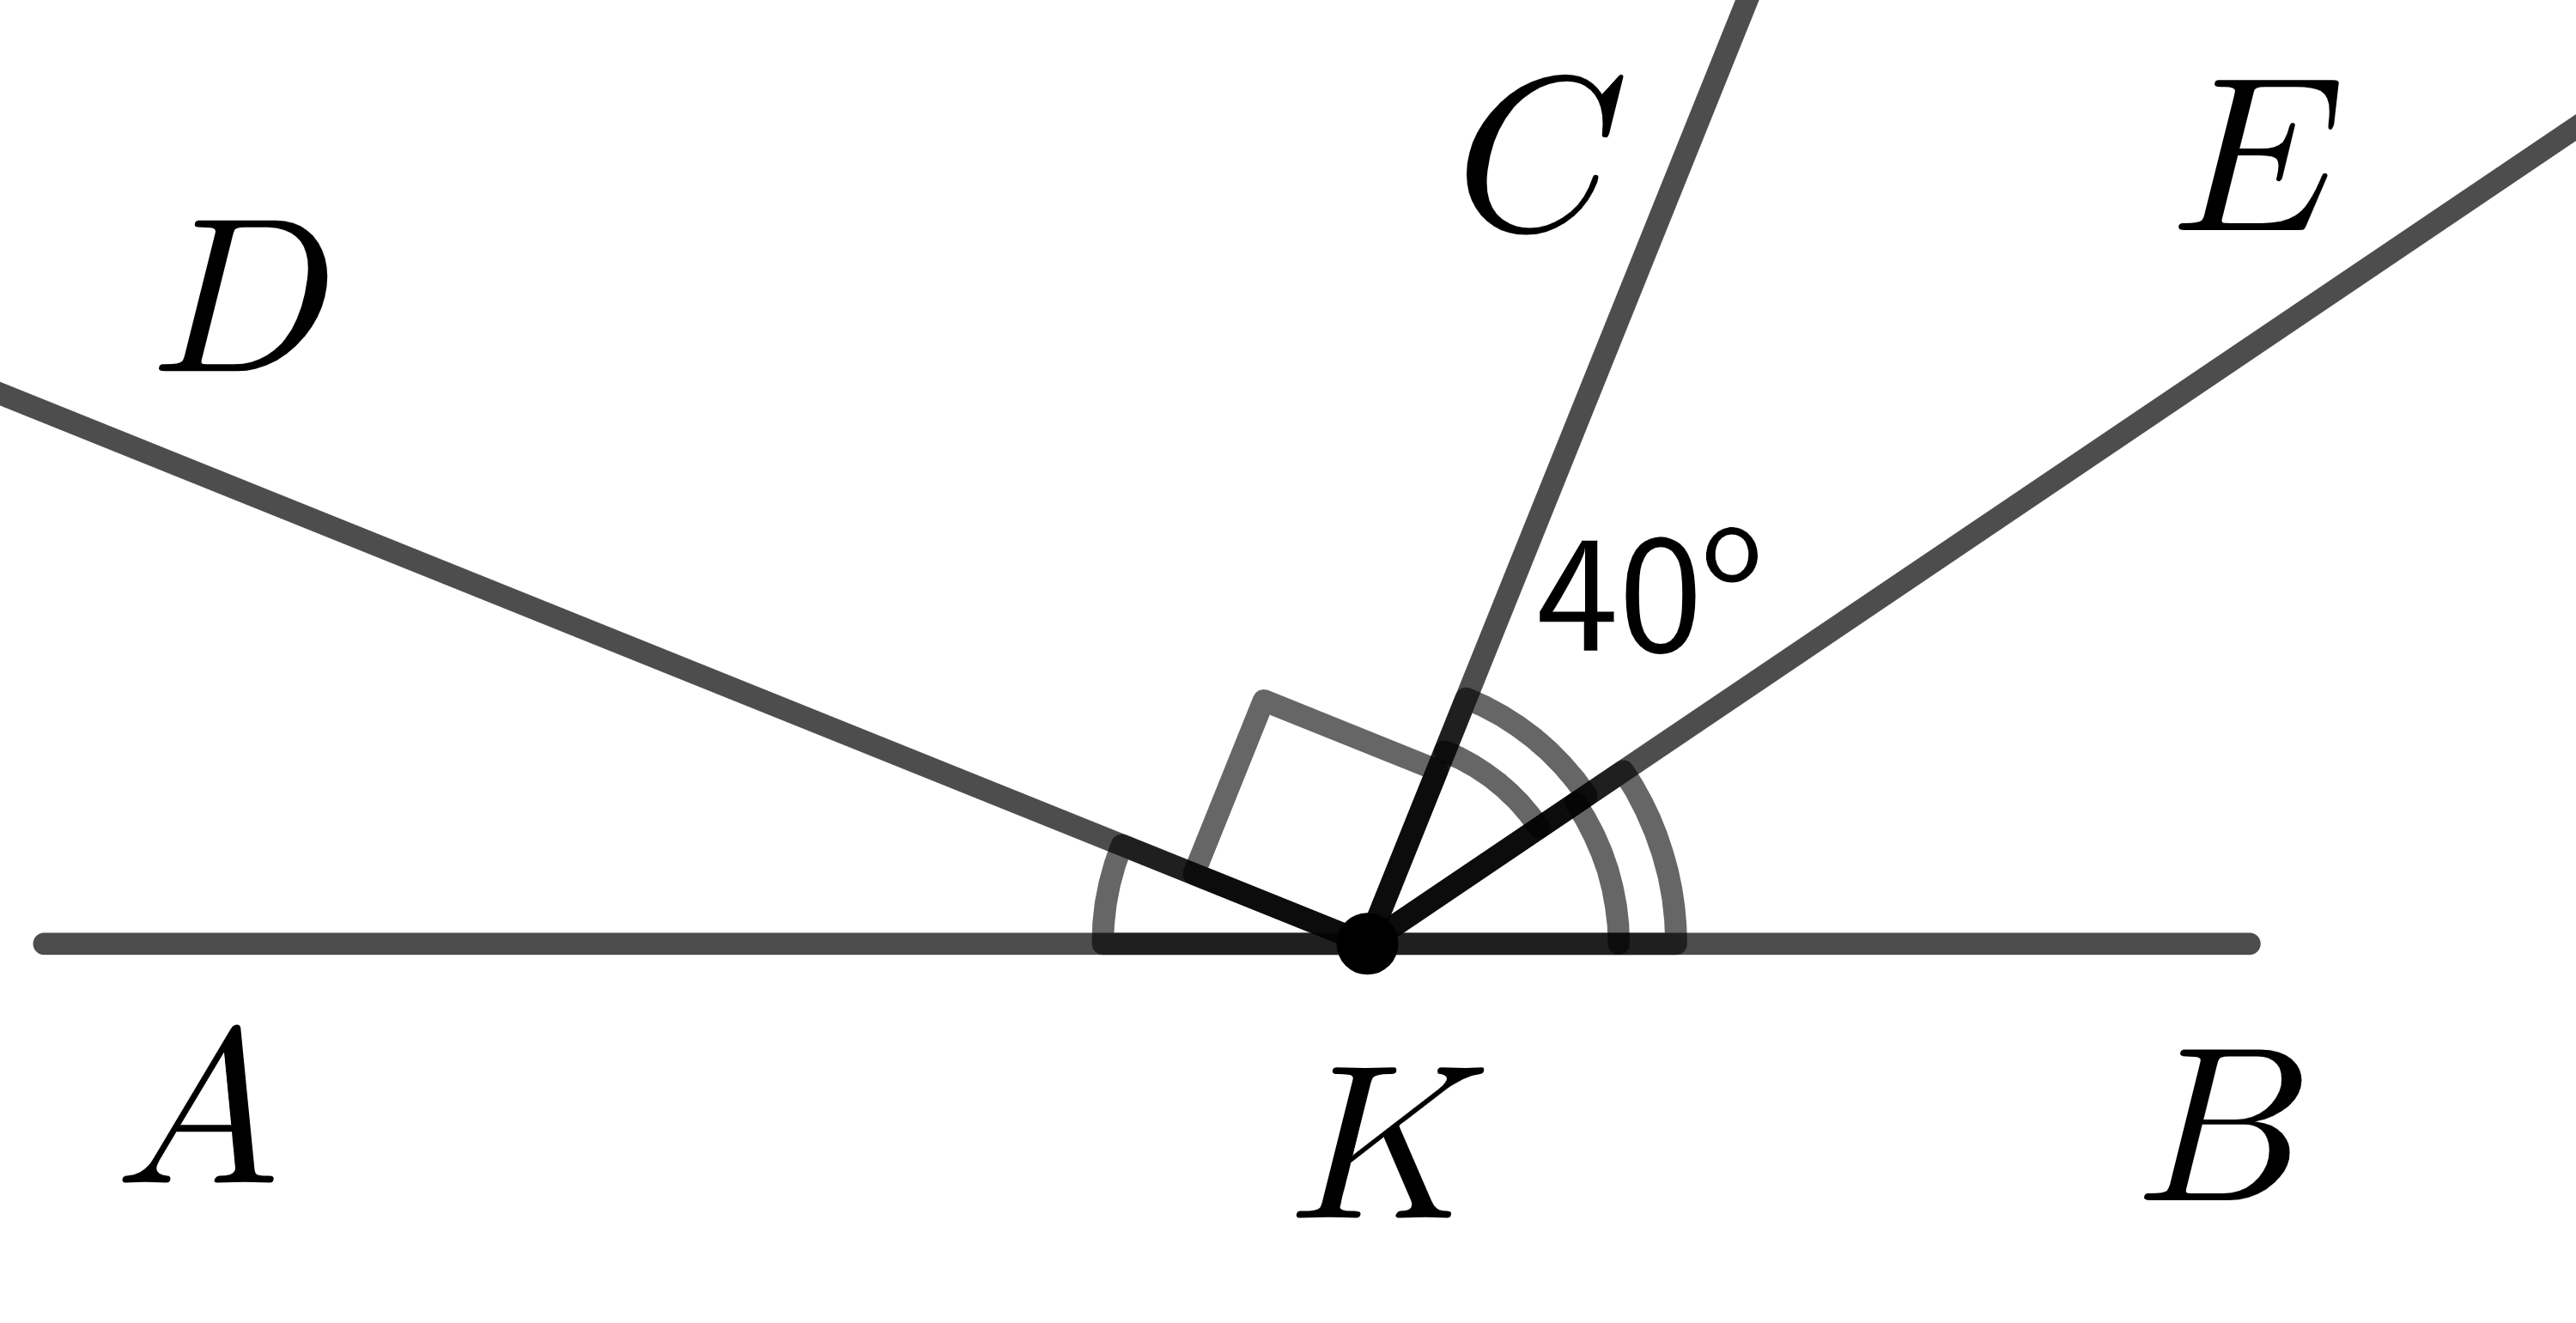
\includegraphics[width=.3\textwidth]{train_exams/20260404/pics/20260404_geom_for_mat_01_v1.png}

\samerowans{\begin{problem}{2a (1 балл)}
Прямые $a$ и $b$ параллельны. По данным чертежа найдите неизвестные углы $x$, $y$ и $z$.
\end{problem}} 

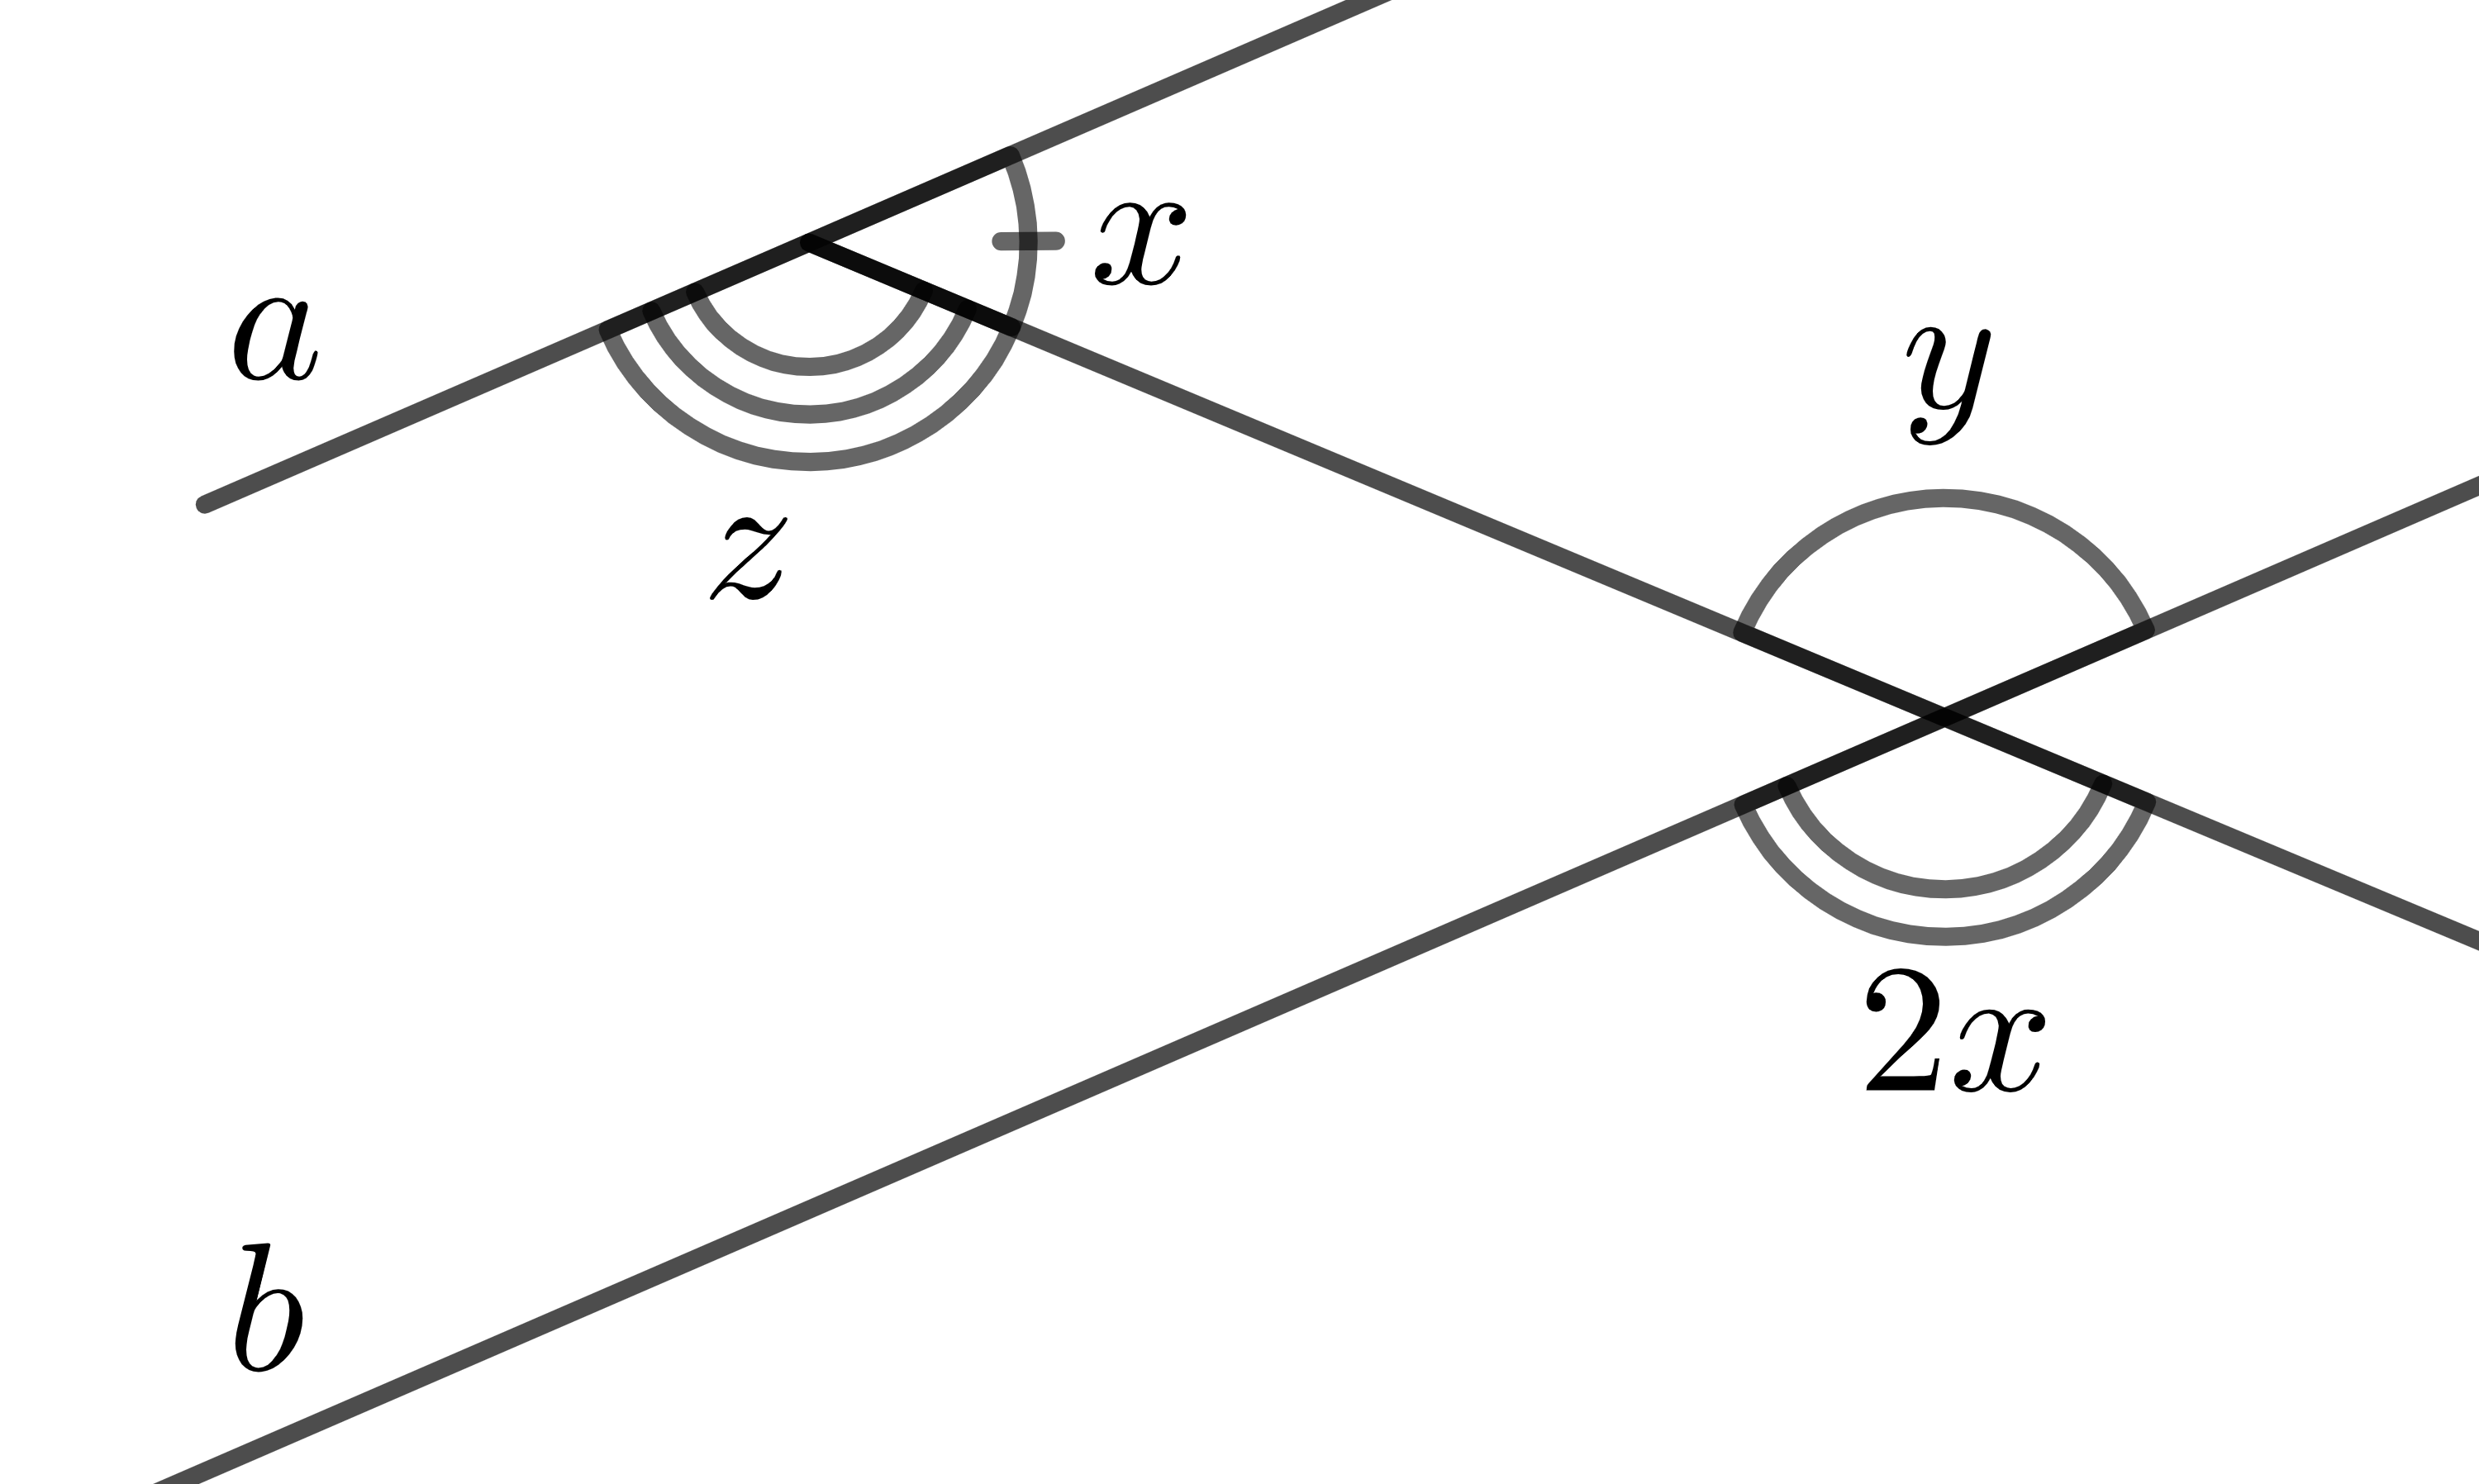
\includegraphics[width=.3\textwidth]{train_exams/20260404/pics/20260404_geom_for_mat_02a_v1.png}

\samerowans{\begin{problem}{2б (2 балла)}
Прямые $a$ и $b$ параллельны. По данным чертежа найдите неизвестные углы $x$, $y$ и $z$.
\end{problem}} 

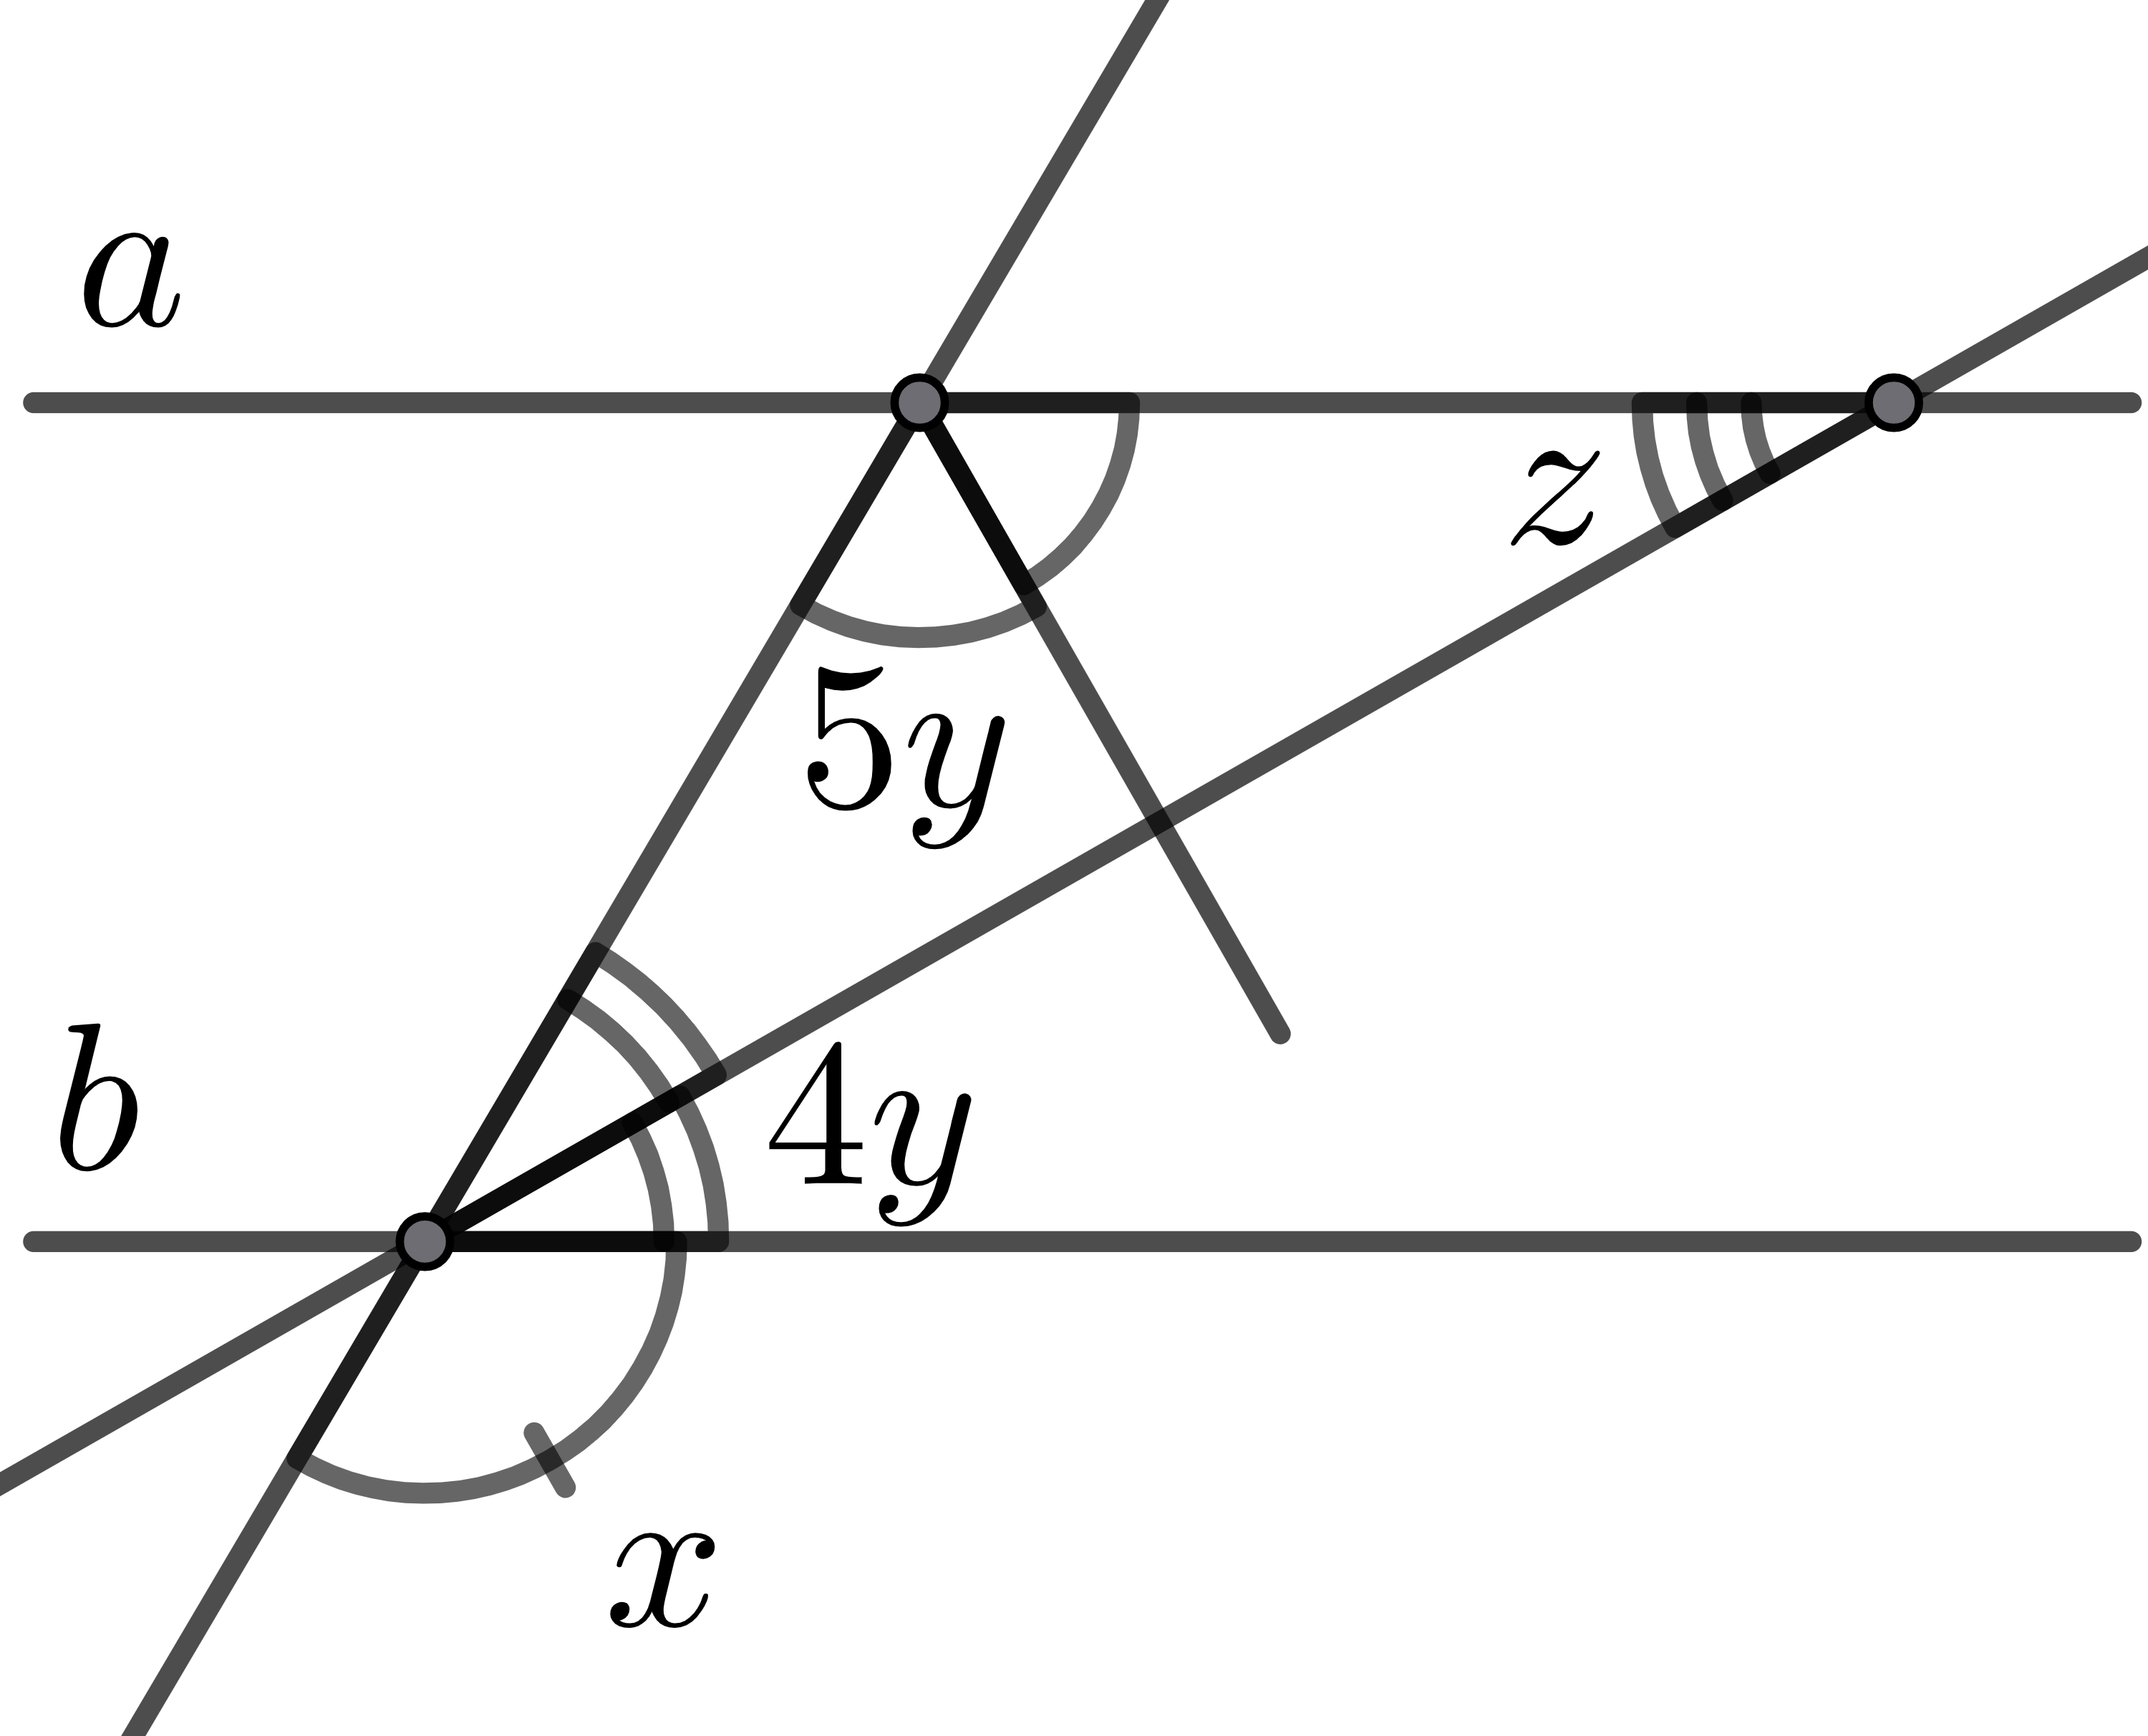
\includegraphics[width=.3\textwidth]{train_exams/20260404/pics/20260404_geom_for_mat_02b_v1.png}

\samerowans{\begin{problem}{3 (1 балл)}
Через точку пересечения биссектрис $\triangle{ABC}$ проведена прямая, параллельная прямой $AC$, пересекающая стороны $AB$ и $BC$ в точках $M$ и $N$ соответственно. $MN=12$, $AM$ на 6 меньше $NC$. Найдите длину $NC$.
\end{problem}} 

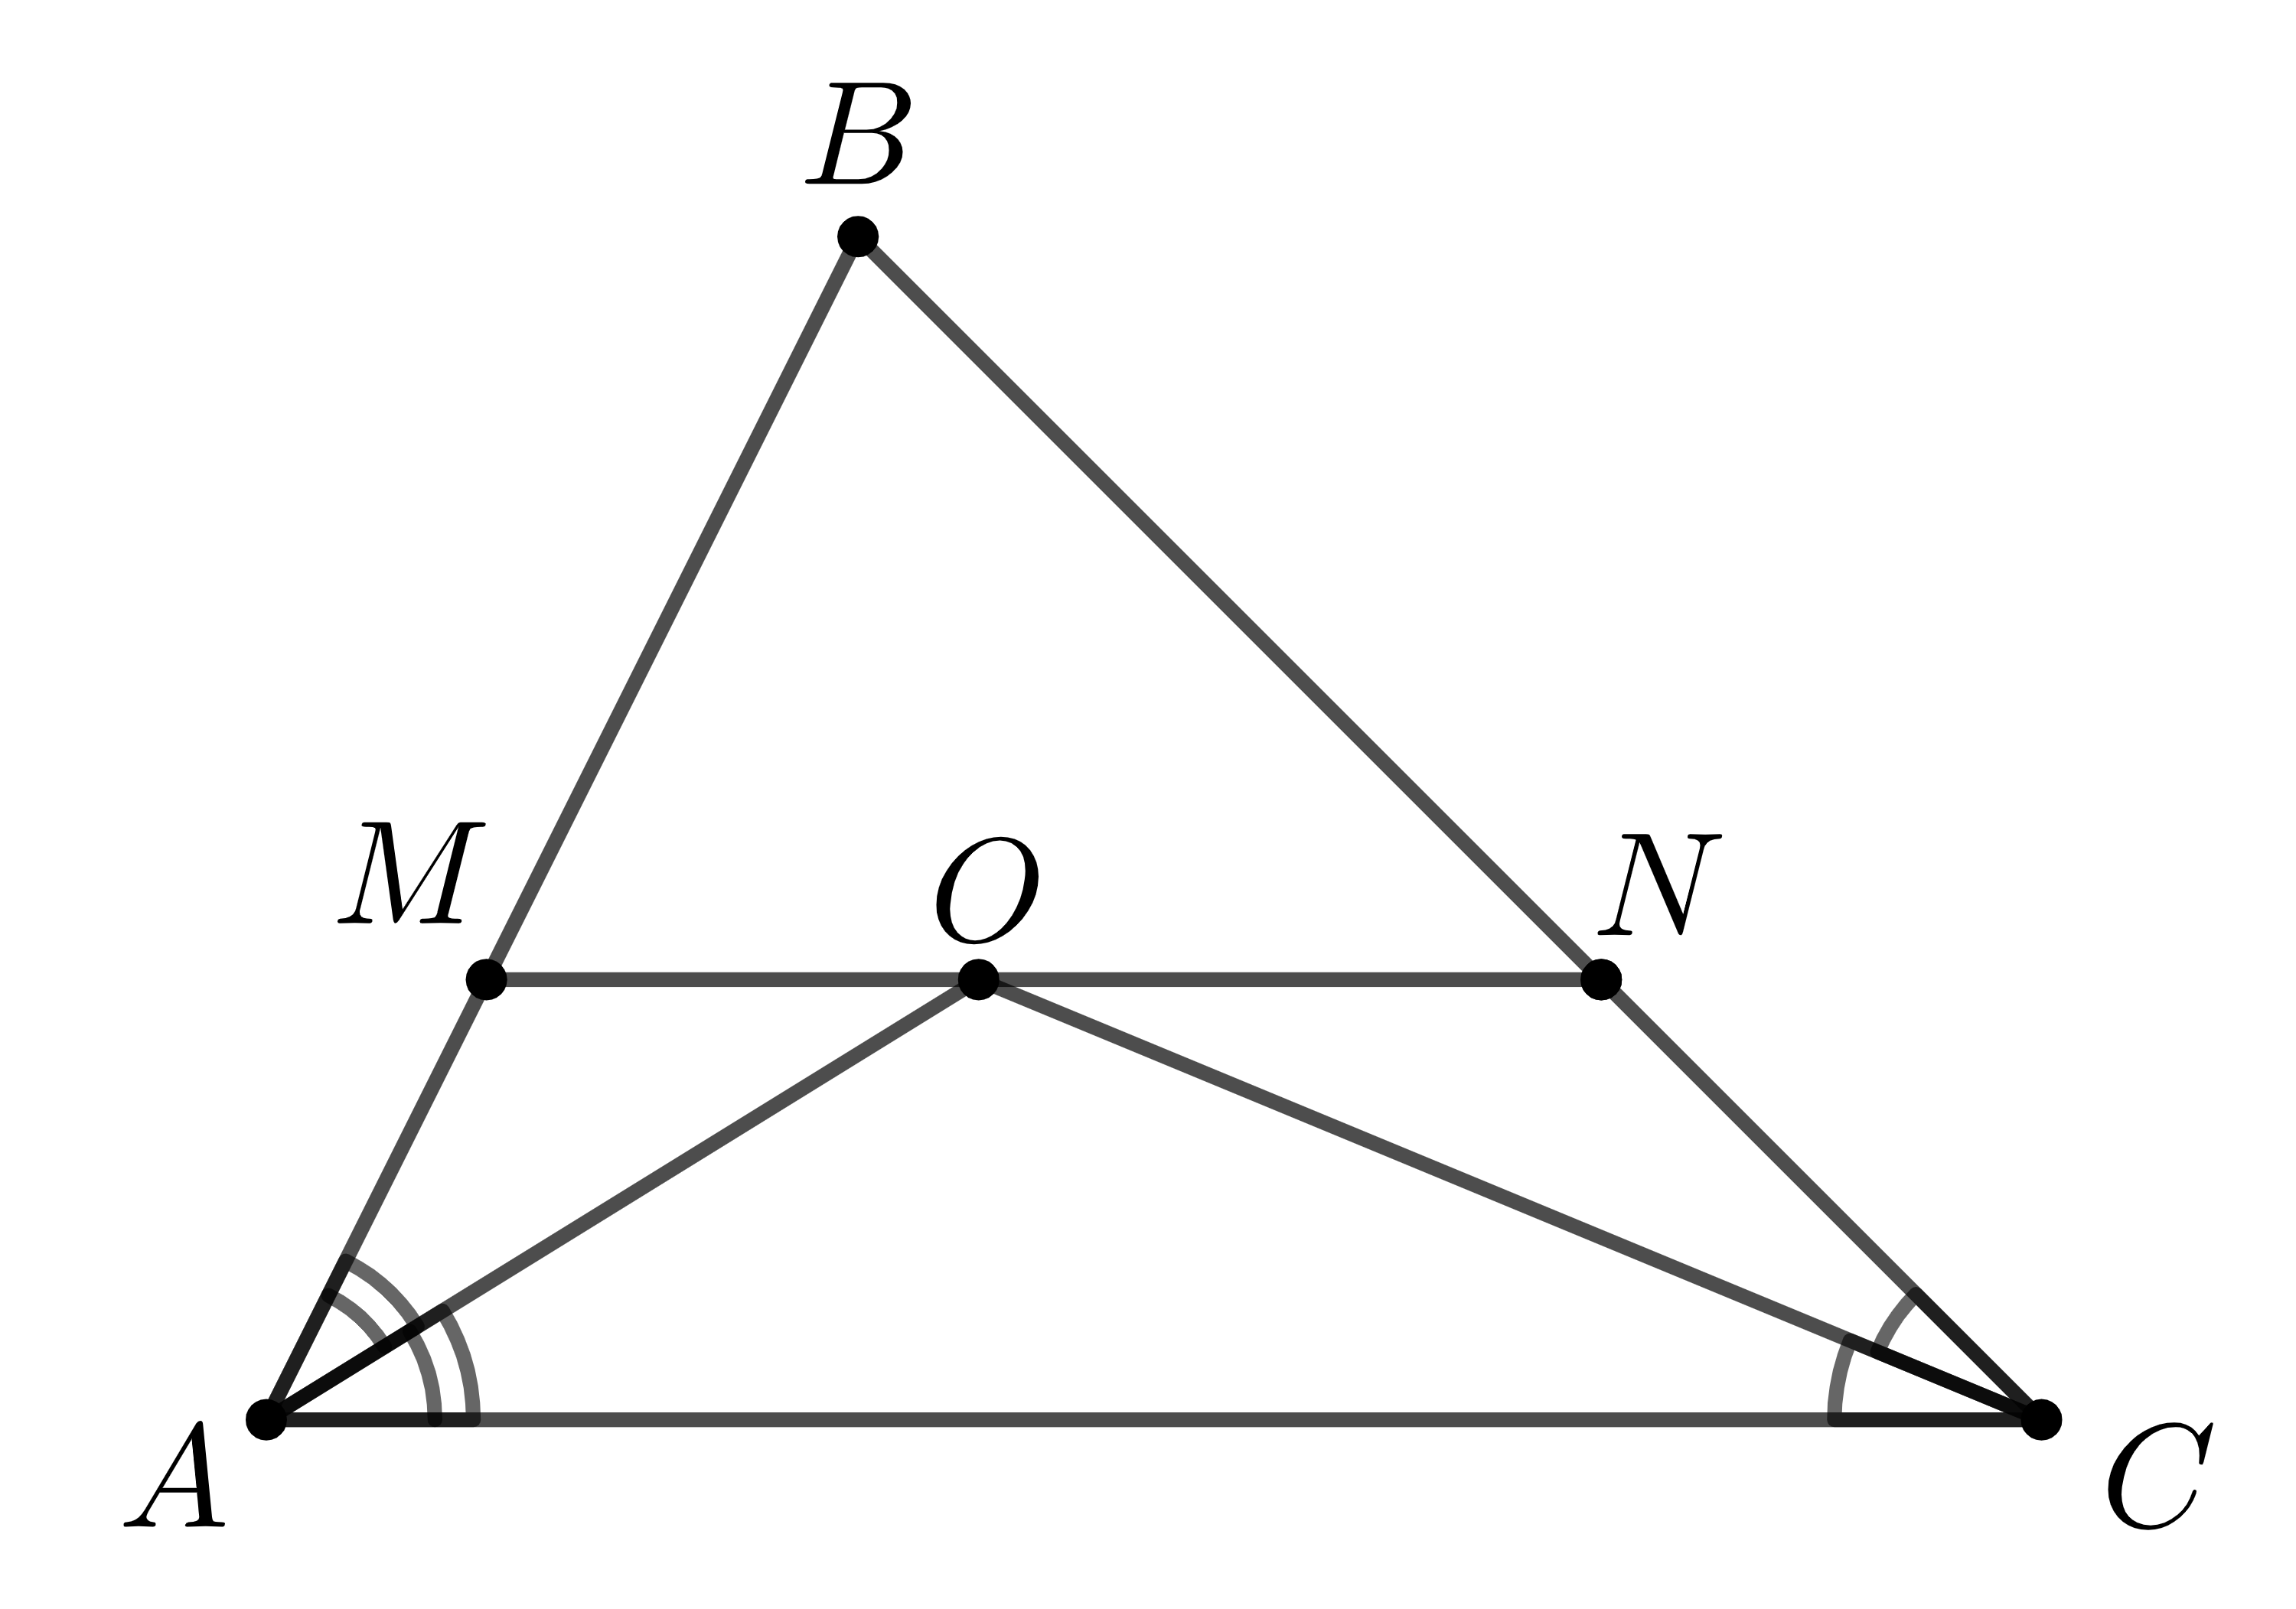
\includegraphics[width=.3\textwidth]{train_exams/20260404/pics/20260404_geom_for_mat_03_v1.png}

\samerowans{\begin{problem}{4 (1 балл)}
Дан равносторонний $\triangle{ABC}$. На стороне $AC$ взята точка $M$ такая, что сумма периметров треугольников $ABM$ и $MBC$ равна 48 см. Найдите длину стороны $\triangle{ABC}$,  если $MB=9\text{ см}$.
\end{problem}} 

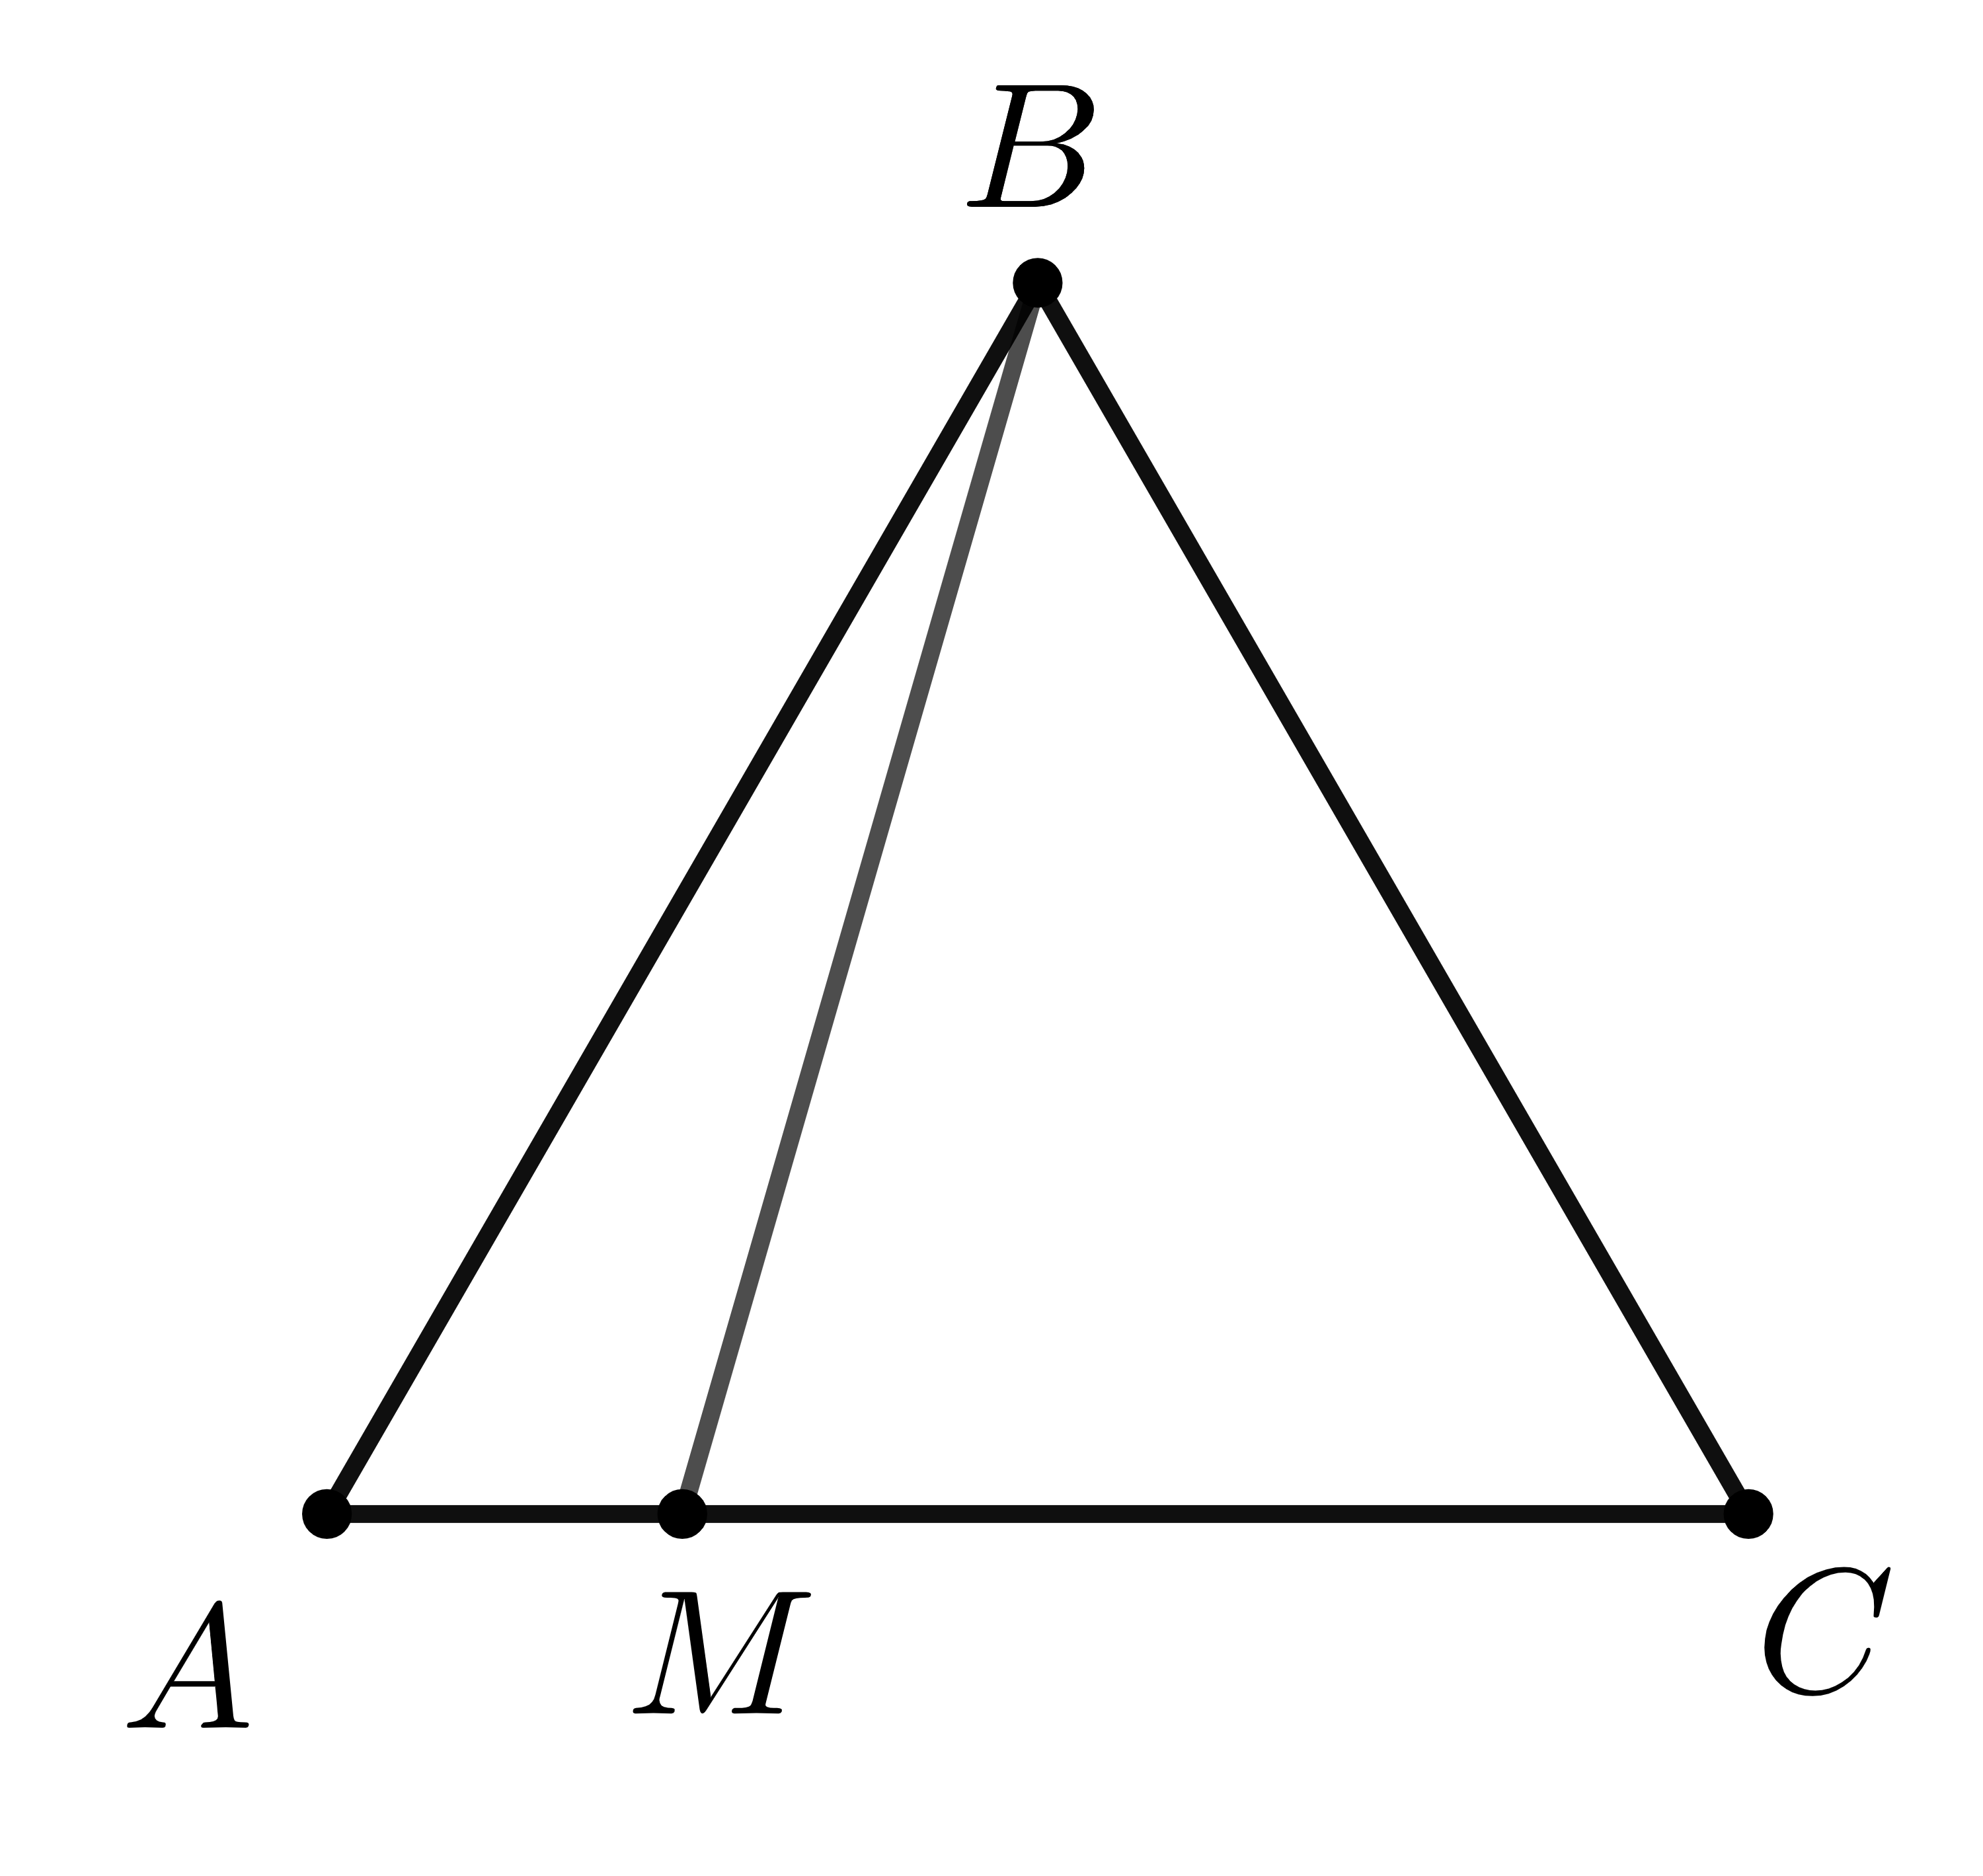
\includegraphics[width=.3\textwidth]{train_exams/20260404/pics/20260404_geom_for_mat_04_v1.png}

\samerowans{\begin{problem}{5 (3 балла)}
Точка $P_1$ --- середина отрезка $CD$. Точка $P_2$ --- середина отрезка $P_1D$. Точка $P_3$ --- середина отрезка $P_2D$. Точка $P_4$ --- середина отрезка $P_3D$. Длина отрезка $P_1P_4=21$ см. Найдите длину отрезка $CD$. 
\end{problem}} 

\samerowans{\begin{problem}{6 (3 балла)}
Выпишите номера верных утверждений. Если верных нет --- напишите 0.
\end{problem}} 

1) Если разность двух сторон и периметр одного треугольника равны разности двух сторон и периметру другого треугольника, то эти треугольники равны. 

2) Если стороны углов соответственно параллельны, то углы равны.

3) Существует прямая, которая перпендикулярна каждой из двух пересекающихся прямых.

4) Медиана треугольника может равняться соседней стороне.


\samerowans{\begin{problem}{7 (3 балла)}
Известно, что $\angle{A} = 35^{\text{o}}$, $\angle{B} = 37^{\text{o}}$, $\angle{C} = 42^{\text{o}}$, $\angle{D} = 45^{\text{o}}$. Найдите $\angle{E}$.
\end{problem}} 

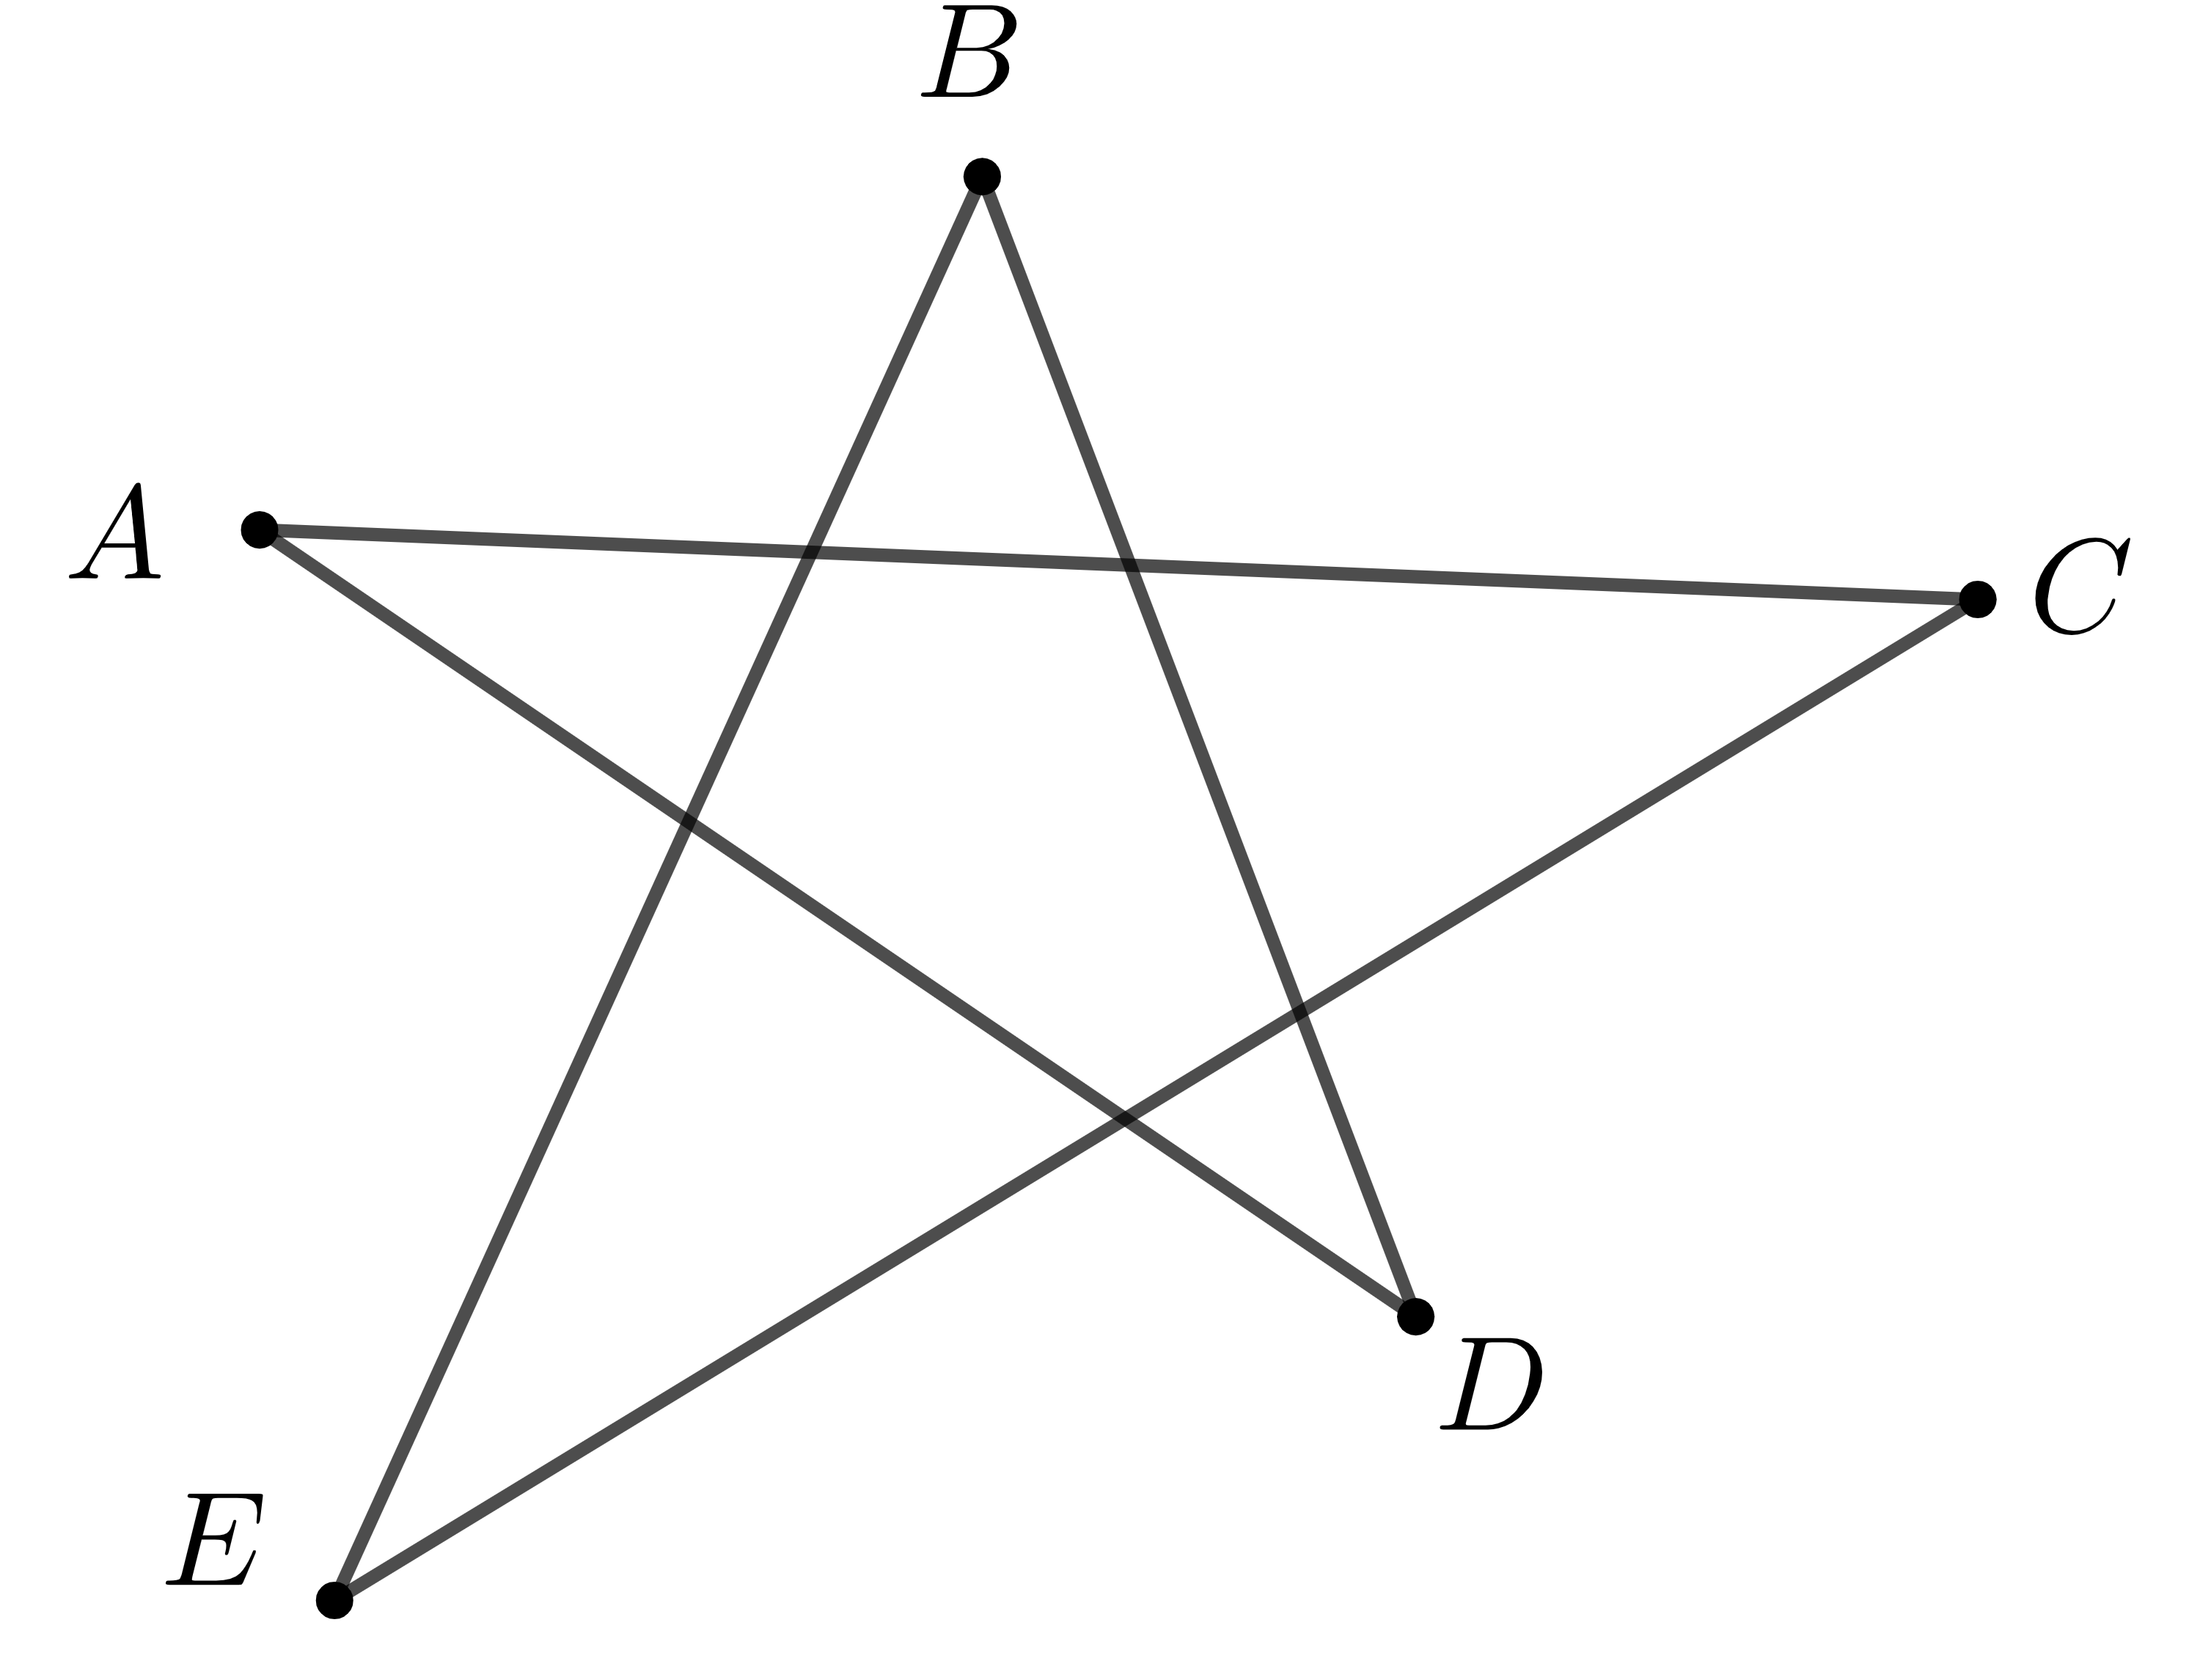
\includegraphics[width=.3\textwidth]{train_exams/20260404/pics/20260404_geom_for_mat_07.png}

\begin{problem}{8 (4 балла)}
На рисунке $\angle{ABC}=90^{\text{o}}$, $\angle{MBA}=45^{\text{o}}$. Докажите, что $\triangle{ABC}$ равнобедренный.
\end{problem}

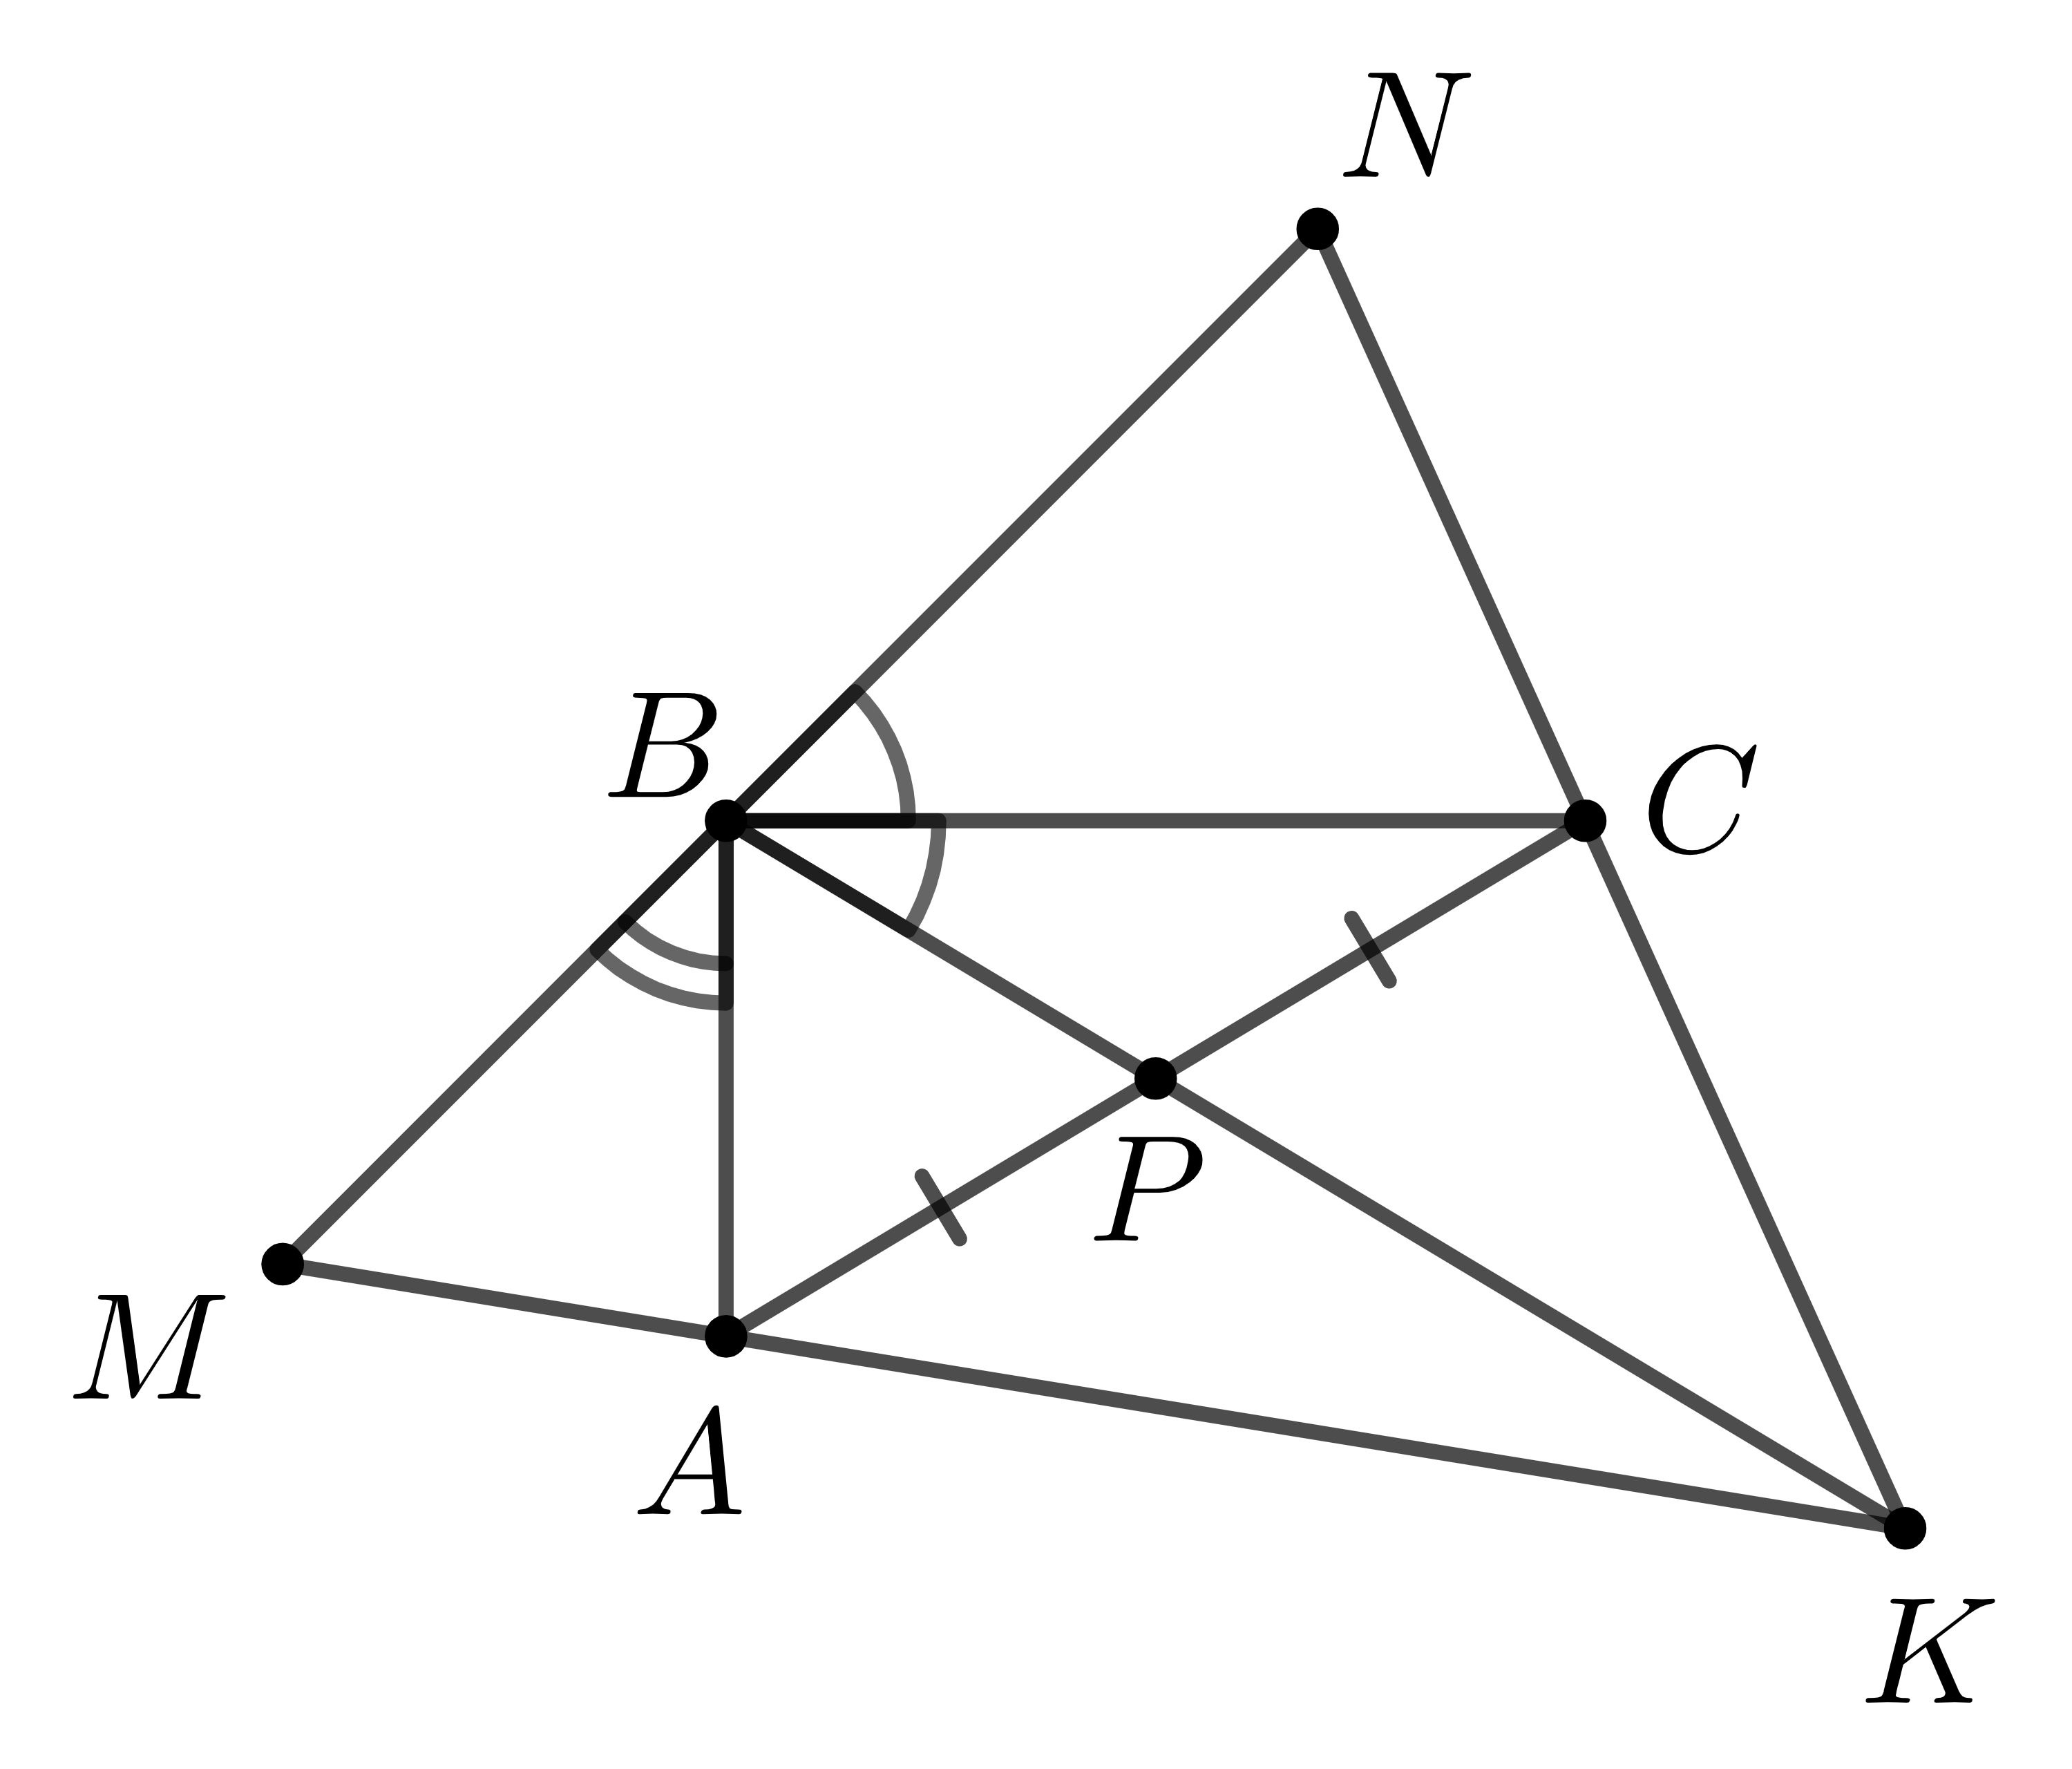
\includegraphics[width=.3\textwidth]{train_exams/20260404/pics/20260404_geom_for_mat_08.png}

\smallskip

\noindent\grid{34}{12}

\smallskip

\begin{problem}{9 (5 баллов)}
Дан четырёхугольник $ABCD$. Известно, что $\angle{CAD}=\angle{DBA}=40^{\text{o}}$, $\angle{CAB=60^{\text{o}}}$, $\angle{CBD}=20^{\text{o}}$. Найдите угол $CDB$.
\end{problem}

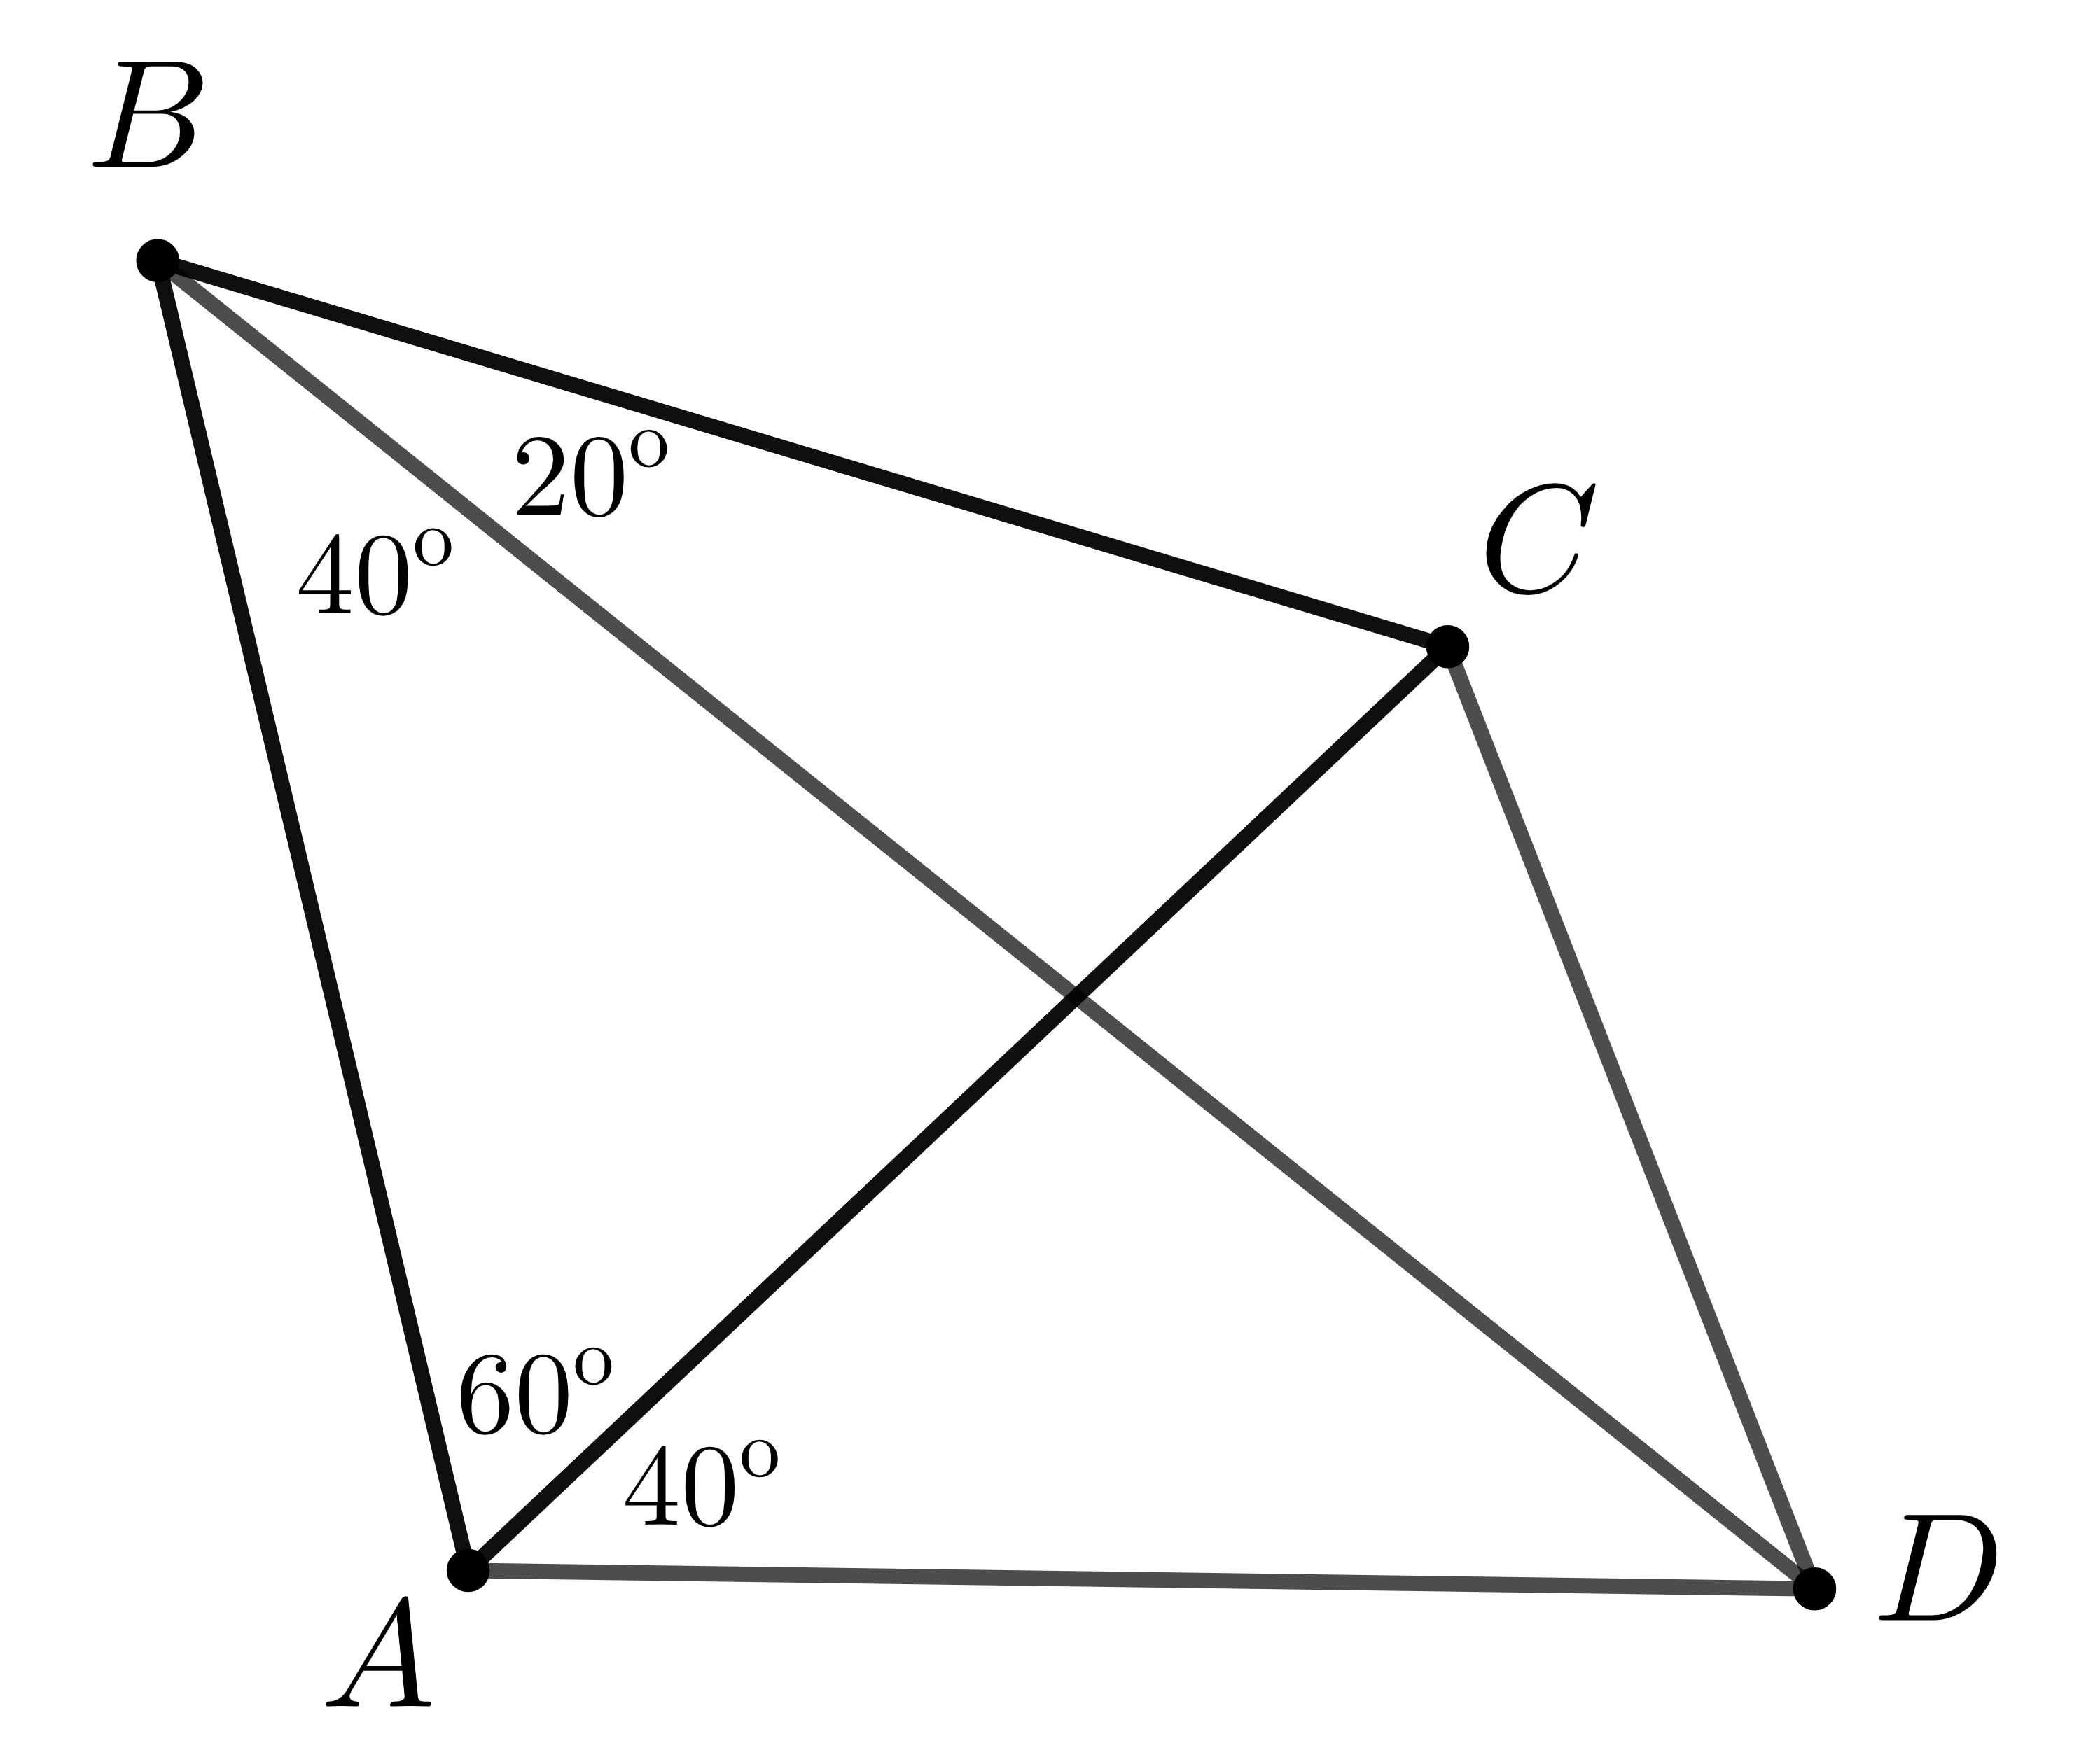
\includegraphics[width=.3\textwidth]{train_exams/20260404/pics/20260404_geom_for_mat_09_v1.png}

\smallskip

\noindent\grid{34}{12}

\smallskip

\begin{problem}{10 (6 баллов)}
На сторонах $BC$ и $CD$ квадрата $ABCD$ взяли точки $K$ и $M$ так, что $BK+DM=MK$. Докажите, что угол  $MAK$ равен $45^{\text{o}}$. 
\end{problem}

\smallskip

\noindent\grid{34}{12}

\smallskip
